\documentclass[english]{SPFShortReport}
\usepackage{subfigure}
\usepackage{spfFigures}
\usepackage{longtable}
\usepackage{url}
\usepackage{gensymb}
\usepackage[yyyymmdd,hhmmss]{datetime}
\reportName{Python calculation for heat pump SIN-11TU}
\reportSubName{Parametric Heat Pump calculation} 
\reportDate{\today \hspace{0.1cm} at: \currenttime \hspace{0.1cm} h} 
\author{Dani Carbonell}
\address{dani.carbonell@solarenergy.ch}
\begin{document}
\begin{table}[!ht]
\begin{small}
\caption{Fitted coefficients for the heat pump.}
\begin{center}
\resizebox{12cm}{!} 
{
\begin{tabular}{l | c c } 
\hline
\hline
Coefficient &Description & \\ 
 & &$[kW]$\\ 
\hline
$PQ_{1}$ & \emph{$1^{st}$ condenser polynomial coefficient}  & 1.0347e+01    \\ 
$PQ_{2}$ & \emph{$2^{st}$ condenser polynomial coefficient}  & 1.1794e+02    \\ 
$PQ_{3}$ & \emph{$3^{st}$ condenser polynomial coefficient}  & 2.9112e+01    \\ 
$PQ_{4}$ & \emph{$4^{st}$ condenser polynomial coefficient}  & -2.0540e+02    \\ 
$PQ_{5}$ & \emph{$5^{st}$ condenser polynomial coefficient}  & 6.8104e+01    \\ 
$PQ_{6}$ & \emph{$6^{st}$ condenser polynomial coefficient}  & -1.4845e+02    \\ 
\hline
$PCOP_{1}$ & \emph{$1^{st}$ COP polynomial coefficient}  & 7.3541e+00    \\ 
$PCOP_{2}$ & \emph{$2^{st}$ COP polynomial coefficient}  & 7.4987e+01    \\ 
$PCOP_{3}$ & \emph{$3^{st}$ COP polynomial coefficient}  & -1.0135e+01    \\ 
$PCOP_{4}$ & \emph{$4^{st}$ COP polynomial coefficient}  & -2.9177e+02    \\ 
$PCOP_{5}$ & \emph{$5^{st}$ COP polynomial coefficient}  & -3.3744e+01    \\ 
$PCOP_{6}$ & \emph{$6^{st}$ COP polynomial coefficient}  & -6.5273e+01    \\ 
\hline
$\dot m_{cond}$ & 1900.00 $[kg/h]$\\ 
$\dot m_{evap}$ & 1900.00 $[kg/h]$\\ 
\hline
$COP_{nom}$ (B0W35)& 4.90 \\ 
$Q_{c,nom}$ (B0W35)& 10.97 kW\\ 
$COP_{nom}$ (B2W35)& 5.19 \\ 
$Q_{c,nom}$ (B2W35)& 11.60 kW\\ 
$COP_{nom}$ (B10W35)& 6.32 \\ 
$Q_{c,nom}$ (B10W35)& 14.19 kW\\ 
\hline
\hline
\end{tabular}
}
\label{CoefTable}
\end{center}
\end{small}
\end{table}
\begin{table}[!ht]
\begin{small}
\caption{Predicting results of the heat pump.}
\begin{center}
\resizebox{12cm}{!} 
{
\begin{tabular}{l | c c c c c c c c c c c } 
\hline
\hline
$T_{evap,in}$ &$T_{evap,out}$ &$T_{cond,in}$ &$T_{cond,out}$ &$COP$ &$Q_{cond}$ &$Q_{evap}$ &$W_{comp}$ &$\dot m_{cond}$ &$\dot m_{evap}$ &$\Delta T_{evap}$ &$\Delta T_{cond}$ \\ 
$^oC$ &$^oC$ &$^oC$ &$^oC$ &$[-]$ &$[kW]$ &$[kW]$ &$[kW]$ &kg/h &kg/h &K &K\\ 
\hline
-7.00 & -10.31 & 26.03 & 30.00 & 4.17 & 8.77 & 6.67 & 2.11 & 1900 & 1900 & 3.3 & 4.0\\ 
-7.00 & -10.17 & 34.77 & 38.75 & 3.65 & 8.80 & 6.39 & 2.41 & 1900 & 1900 & 3.2 & 4.0\\ 
-7.00 & -9.83 & 43.63 & 47.50 & 3.00 & 8.56 & 5.71 & 2.85 & 1900 & 1900 & 2.8 & 3.9\\ 
-7.00 & -9.19 & 52.62 & 56.25 & 2.21 & 8.03 & 4.40 & 3.63 & 1900 & 1900 & 2.2 & 3.6\\ 
-7.00 & -7.76 & 61.72 & 65.00 & 1.27 & 7.26 & 1.54 & 5.72 & 1900 & 1900 & 0.8 & 3.3\\ 
-4.00 & -7.79 & 25.61 & 30.00 & 4.65 & 9.71 & 7.62 & 2.09 & 1900 & 1900 & 3.8 & 4.4\\ 
-4.00 & -7.62 & 34.37 & 38.75 & 4.05 & 9.69 & 7.30 & 2.39 & 1900 & 1900 & 3.6 & 4.4\\ 
-4.00 & -7.25 & 43.25 & 47.50 & 3.31 & 9.39 & 6.55 & 2.84 & 1900 & 1900 & 3.3 & 4.2\\ 
-4.00 & -6.57 & 52.27 & 56.25 & 2.42 & 8.81 & 5.17 & 3.63 & 1900 & 1900 & 2.6 & 4.0\\ 
-4.00 & -5.09 & 61.39 & 65.00 & 1.38 & 7.98 & 2.20 & 5.78 & 1900 & 1900 & 1.1 & 3.6\\ 
-1.00 & -5.27 & 25.18 & 30.00 & 5.14 & 10.67 & 8.59 & 2.08 & 1900 & 1900 & 4.3 & 4.8\\ 
-1.00 & -5.08 & 33.96 & 38.75 & 4.44 & 10.59 & 8.21 & 2.38 & 1900 & 1900 & 4.1 & 4.8\\ 
-1.00 & -4.67 & 42.87 & 47.50 & 3.61 & 10.24 & 7.40 & 2.84 & 1900 & 1900 & 3.7 & 4.6\\ 
-1.00 & -3.95 & 51.91 & 56.25 & 2.63 & 9.60 & 5.95 & 3.65 & 1900 & 1900 & 3.0 & 4.3\\ 
-1.00 & -2.43 & 61.06 & 65.00 & 1.49 & 8.72 & 2.87 & 5.85 & 1900 & 1900 & 1.4 & 3.9\\ 
2.00 & -2.75 & 24.74 & 30.00 & 5.62 & 11.64 & 9.57 & 2.07 & 1900 & 1900 & 4.8 & 5.3\\ 
2.00 & -2.53 & 33.54 & 38.75 & 4.83 & 11.51 & 9.13 & 2.38 & 1900 & 1900 & 4.5 & 5.2\\ 
2.00 & -2.10 & 42.48 & 47.50 & 3.91 & 11.10 & 8.26 & 2.84 & 1900 & 1900 & 4.1 & 5.0\\ 
2.00 & -1.34 & 51.54 & 56.25 & 2.83 & 10.40 & 6.73 & 3.67 & 1900 & 1900 & 3.3 & 4.7\\ 
2.00 & 0.24 & 60.71 & 65.00 & 1.60 & 9.48 & 3.54 & 5.93 & 1900 & 1900 & 1.8 & 4.3\\ 
5.00 & -0.24 & 24.29 & 30.00 & 6.10 & 12.63 & 10.56 & 2.07 & 1900 & 1900 & 5.2 & 5.7\\ 
5.00 & 0.00 & 33.12 & 38.75 & 5.22 & 12.45 & 10.06 & 2.38 & 1900 & 1900 & 5.0 & 5.6\\ 
5.00 & 0.47 & 42.08 & 47.50 & 4.21 & 11.98 & 9.13 & 2.85 & 1900 & 1900 & 4.5 & 5.4\\ 
5.00 & 1.26 & 51.17 & 56.25 & 3.03 & 11.23 & 7.53 & 3.70 & 1900 & 1900 & 3.7 & 5.1\\ 
5.00 & 2.90 & 60.37 & 65.00 & 1.70 & 10.25 & 4.22 & 6.03 & 1900 & 1900 & 2.1 & 4.6\\ 
8.00 & 2.26 & 23.84 & 30.00 & 6.58 & 13.63 & 11.56 & 2.07 & 1900 & 1900 & 5.7 & 6.2\\ 
8.00 & 2.53 & 32.69 & 38.75 & 5.61 & 13.40 & 11.01 & 2.39 & 1900 & 1900 & 5.5 & 6.1\\ 
8.00 & 3.03 & 41.68 & 47.50 & 4.50 & 12.88 & 10.01 & 2.86 & 1900 & 1900 & 5.0 & 5.8\\ 
8.00 & 3.86 & 50.79 & 56.25 & 3.23 & 12.07 & 8.34 & 3.73 & 1900 & 1900 & 4.1 & 5.5\\ 
8.00 & 5.56 & 60.01 & 65.00 & 1.80 & 11.04 & 4.91 & 6.13 & 1900 & 1900 & 2.4 & 5.0\\ 
11.00 & 4.76 & 23.37 & 30.00 & 7.05 & 14.65 & 12.58 & 2.08 & 1900 & 1900 & 6.2 & 6.6\\ 
11.00 & 5.06 & 32.25 & 38.75 & 5.99 & 14.36 & 11.97 & 2.40 & 1900 & 1900 & 5.9 & 6.5\\ 
11.00 & 5.58 & 41.27 & 47.50 & 4.79 & 13.79 & 10.91 & 2.88 & 1900 & 1900 & 5.4 & 6.2\\ 
11.00 & 6.45 & 50.40 & 56.25 & 3.43 & 12.93 & 9.16 & 3.77 & 1900 & 1900 & 4.5 & 5.8\\ 
11.00 & 8.22 & 59.64 & 65.00 & 1.90 & 11.85 & 5.61 & 6.24 & 1900 & 1900 & 2.8 & 5.4\\ 
14.00 & 7.24 & 22.90 & 30.00 & 7.53 & 15.69 & 13.61 & 2.08 & 1900 & 1900 & 6.8 & 7.1\\ 
14.00 & 7.57 & 31.81 & 38.75 & 6.38 & 15.35 & 12.94 & 2.41 & 1900 & 1900 & 6.4 & 6.9\\ 
14.00 & 8.13 & 40.84 & 47.50 & 5.08 & 14.72 & 11.82 & 2.90 & 1900 & 1900 & 5.9 & 6.7\\ 
14.00 & 9.04 & 50.01 & 56.25 & 3.62 & 13.80 & 9.99 & 3.81 & 1900 & 1900 & 5.0 & 6.2\\ 
14.00 & 10.86 & 59.27 & 65.00 & 1.99 & 12.67 & 6.31 & 6.36 & 1900 & 1900 & 3.1 & 5.7\\ 
17.00 & 9.73 & 22.43 & 30.00 & 8.00 & 16.74 & 14.65 & 2.09 & 1900 & 1900 & 7.3 & 7.6\\ 
17.00 & 10.08 & 31.36 & 38.75 & 6.76 & 16.35 & 13.93 & 2.42 & 1900 & 1900 & 6.9 & 7.4\\ 
17.00 & 10.67 & 40.42 & 47.50 & 5.37 & 15.66 & 12.74 & 2.92 & 1900 & 1900 & 6.3 & 7.1\\ 
17.00 & 11.62 & 49.61 & 56.25 & 3.81 & 14.69 & 10.84 & 3.85 & 1900 & 1900 & 5.4 & 6.6\\ 
17.00 & 13.51 & 58.89 & 65.00 & 2.09 & 13.51 & 7.03 & 6.48 & 1900 & 1900 & 3.5 & 6.1\\ 
20.00 & 12.20 & 21.95 & 30.00 & 8.47 & 17.81 & 15.71 & 2.10 & 1900 & 1900 & 7.8 & 8.1\\ 
20.00 & 12.59 & 30.90 & 38.75 & 7.14 & 17.36 & 14.93 & 2.43 & 1900 & 1900 & 7.4 & 7.9\\ 
20.00 & 13.21 & 39.98 & 47.50 & 5.65 & 16.62 & 13.68 & 2.94 & 1900 & 1900 & 6.8 & 7.5\\ 
20.00 & 14.19 & 49.19 & 56.25 & 4.00 & 15.60 & 11.70 & 3.90 & 1900 & 1900 & 5.8 & 7.1\\ 
20.00 & 16.14 & 58.50 & 65.00 & 2.18 & 14.37 & 7.77 & 6.60 & 1900 & 1900 & 3.9 & 6.5\\ 
\hline
\hline
\end{tabular}
}
\label{ResultsTable}
\end{center}
\end{small}
\end{table}
\begin{figure}[!ht]
\begin{center}
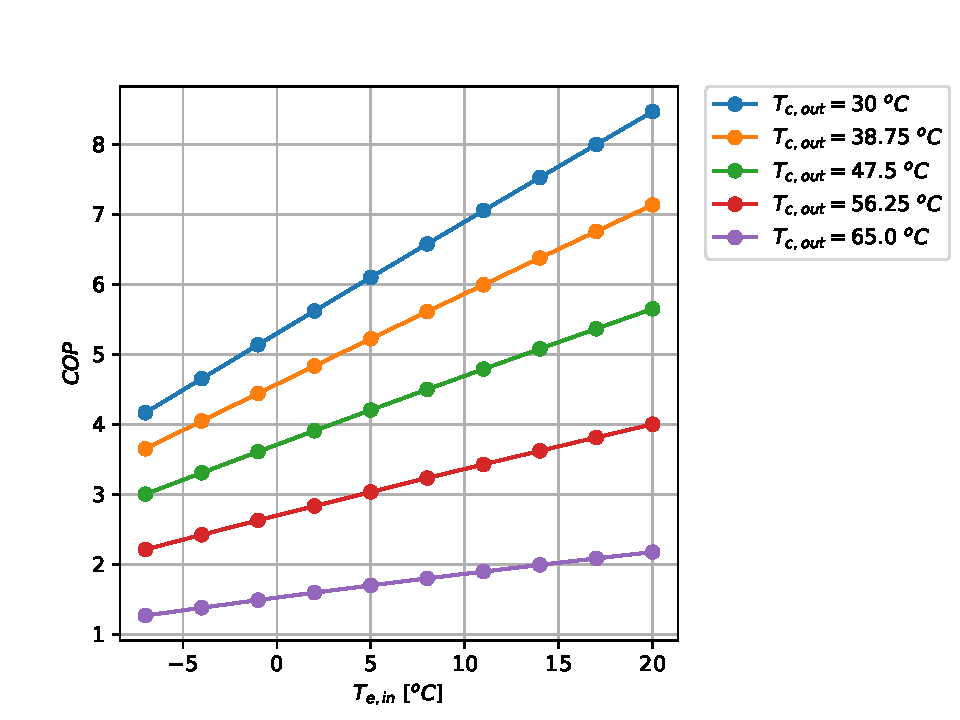
\includegraphics[width=1\textwidth]{C:/Daten/spfPackages/GIT/spfTrnsysFiles/HeatPump/BrineToWater/Walter Meier/SIN-11TU/SIN-11TU-Cop.pdf}
\caption{COP Results for the heat pump at the selected points}
\label{COPFig}
\end{center}
\end{figure}
\begin{figure}[!ht]
\begin{center}
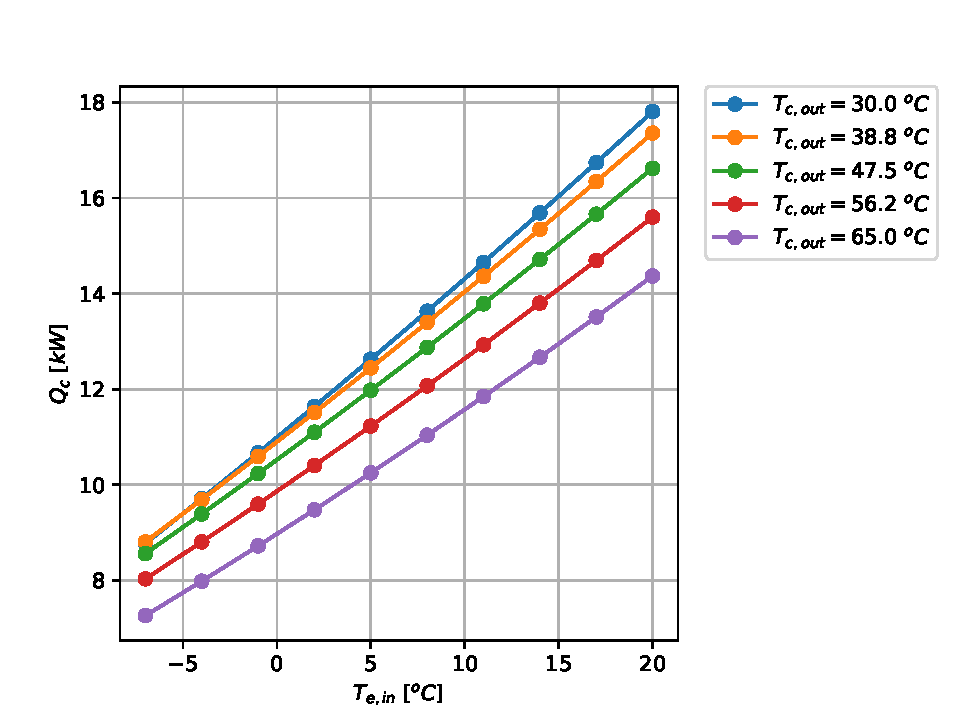
\includegraphics[width=1\textwidth]{C:/Daten/spfPackages/GIT/spfTrnsysFiles/HeatPump/BrineToWater/Walter Meier/SIN-11TU/SIN-11TU-Qc.pdf}
\caption{$Q_c$ Results for the heat pump at the selected points}
\label{QcFig}
\end{center}
\end{figure}
\end{document}
